\ac{sturesy} ist der Name einer Software, die im Rahmen der Bachelorarbeit von Wolf Posdorfer im Jahr 2012 an der Universität Hamburg entstanden ist. Der Name StuReSy ist ein Akronym für „Student Response System“. StuReSy wurde erfolgreich und viele Jahre an der Universität Hamburg und HAW Hamburg eingesetzt. Die Qualität und der Umfang der Software sind für eine Bachelorarbeit beeindruckend.

StuReSy besteht aus zwei Komponenten:
\begin{itemize}
    \item \textbf{Server-Komponente}: In PHP geschrieben, agiert gleichzeitig als Client-Komponente für die Abstimmungs-Teilenehmer (kann über den Browser aufgerufen werden) und Administrations-Oberfläche. Benötigt eine relationale SQL-Datenbank.
    \item \textbf{Editor-Komponente}: In Java geschrieben. Um Fragen zu erstellen und zu bearbeiten.
\end{itemize}

Der StuReSy-Editor verfügt über folgende Haupt-Funktionen bzw. Programmteile:
\begin{itemize}
    \item \textbf{Abstimmung}: Durchführung einer Umfrage
    \item \textbf{Fragen-Editor}: Erstellung und Bearbeitung von Fragesätzen.
    \item \textbf{Abstimmungs-Analyse}: Auswerten von Abstimmungs-Ergebnissen im Nachhinein.
\end{itemize}

\begin{figure}[H]
    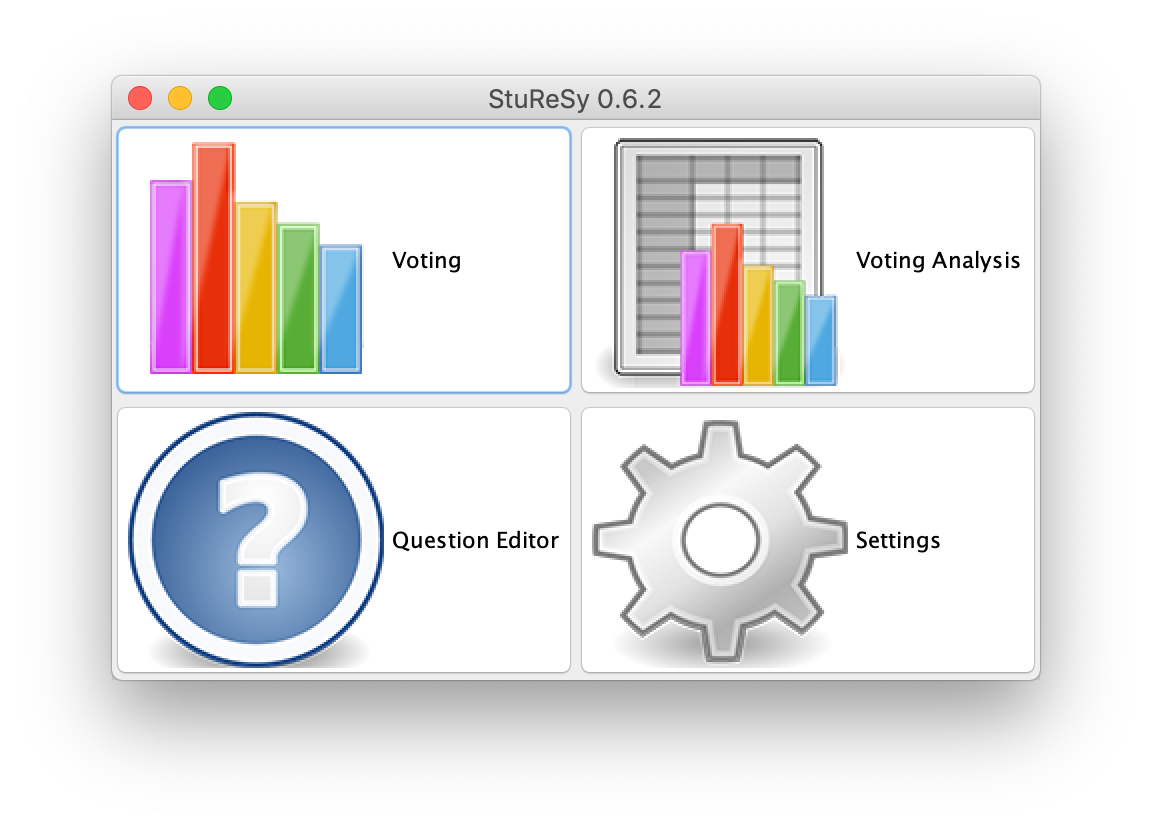
\includegraphics[width=16cm]{chapter/bewertung/bilder/StuReSy_Hauptmenue.png}
    \centering
    \caption{Hauptmenü der StuReSy-Editor-Komponente.}
    \label{Abbildung 2.1}
\end{figure}


Auch wenn StuReSy erfolgreich im Hochschul-Alltag verwendet wurde, so gibt es trotzdem einige konzeptionelle Nachteile:
\begin{itemize}
    \item \textbf{Software-Download und JVM notwendig}: Um StuReSy administrativ einsetzen zu können, muss eine Java-Software heruntergeladen werden und eine JVM muss auf dem jeweiligen System vorhanden sein. Eine Administration vom Tablet oder Smartphone ist damit nur schwer möglich.
    \item \textbf{Server notwendig}: Um StuReSy betreiben zu können, wird eine Server-Instanz benötigt. Diese muss von der jeweiligen Institution oder einem Dozenten aufgesetzt und gewartet werden.
\end{itemize}

Neben den konzeptionellen Problemen gibt es auch Probleme mit der konkreten Implementierung von StuReSy:\newline
\textbf{Mangelnde Formatierungsmöglichkeiten für Software-Quelltext}: In der Praxis wird StuReSy vor allem in Informatik-Veranstaltungen eingesetzt. Dort werden oft Fragen zu Quelltext-Ausschnitten gestellt. Die Darstellung dieser Quelltexte in StuReSy ist schwierig. Obwohl StuReSy die Formatierung von Fragen mittels HTML zulässt ist es nicht leicht hier ordentliche Ergebnisse zu erzielen, ohne manuell den HTML-Code zu editieren. Zentrierte Text-Ausrichtung für Quelltext liest sich sehr schwer. Linksbündige Ausrichtung wirkt oft sehr deplatziert im Gegensatz zur zentrierten Fragestellung.
